\documentclass[a4paper,10pt,twoside]{report}
\usepackage[T1]{fontenc}
\usepackage[frenchb]{babel} %active le mode français
\usepackage[latin1,utf8]{inputenc} % Mettre des accents
\usepackage[top=2cm , bottom=2cm , left=2cm , right=2cm]{geometry} %propriétés de notre page
\usepackage{amsmath} %liste de symboles et applications mathématiques
\usepackage{amsfonts} %idem
\usepackage{color} %Permet d'utiliser la couleur dans nos documents
\usepackage[usenames,dvipsnames]{xcolor}
\usepackage{listings} %Paquet de coloration syntaxique (langages)
\usepackage{hyperref} % Créer des liens et des signets 
\usepackage[babel=true]{csquotes} %permet les quotations (guillemets)
\usepackage{graphicx} %Importation d'image
\usepackage{fancyhdr} %en-tête et pieds de page+
\usepackage{lastpage} %permet d'obtenir le nombre total de page
\usepackage{multido}
%\usepackage{eurosym}
\usepackage{listingsutf8}
\usepackage{tikz}
\usepackage{ulem}
\usepackage{colortbl} %permet de mettre de personnaliser les colones des tabular
\usepackage{pdfpages}
\usepackage{appendix} %annexes
\setlength{\headheight}{15pt}
\lstset{language=C,
    breaklines=true,
	numbers=left,
	keywordstyle=\color{blue},
	commentstyle=\color{Gray},
	stringstyle=\color{red},
	tabsize=4,
	framexleftmargin=7mm,
	frame=single
	}
% Informations du rapport
\title {Rapport de TP \\ Mes\_meilleurs\_trajets.com}
\author {Quentin Tonneau - Guillaume Goisque}
\date{}
\renewcommand{\thesection}{\arabic{section}}
%Propriétés des liens
\hypersetup{
colorlinks=true, %colorise les liens  
urlcolor= blue, %couleur des hyperliens 
linkcolor= blue,%couleur des liens internes
citecolor=black
} 
%\setlength{\parindent}{0cm}
\addto\captionsfrench{
	\renewcommand{\chaptername}{Partie}
}

\fancypagestyle{plain}
{

	\fancyhead{}
	\fancyfoot{}
	\fancyfoot[LO RE]{\textit{Q.Tonneau - G.Goisque}}
	\lhead{X7IO010}
	\rhead{Université de Nantes}
	\chead{Mes\_meilleurs\_trajets.com}
	\fancyfoot[LE]{\thepage}
	\fancyfoot[RO]{\thepage}
}
\begin{document}
\thispagestyle{empty}
\Large{\uline{
\noindent Guillaume Goisque}


\uline{Quentin Tonneau}}
\vfill
\begin{center}
\Huge{
 Rapport de Travaux Pratiques\\
 \textbf{Mes\_meilleurs\_trajets.com}}
 \vfill
 \includegraphics[width=0.75\textwidth]{logo_univ_nantes.png}
 \vfill
\end{center}
X7IO020 \hfill Décembre 2012
%\newpage \pagestyle{empty}~
\tableofcontents
\newpage
\pagestyle{plain}
\chapter{Introduction}
Ce projet traite d'un cas de réponse à la demande d'une compagnie ferroviaire souhaitant disposer d'un programme permettant aux voyageurs d'effectuer une recherche de trajet entre deux gares, selon deux critères : le temps de trajet et le prix du voyage.\\
Le programme doit contenir une interface ergonomique dans laquelle le client indiquera ses choix concernant le trajet : ville de départ, ville d'arrivée, à partir de quelle heure, la classe, ainsi que le choix du critère qu'il souhaite minimiser : le temps de trajet, le prix, ou un mixte des deux critères.\\
Le programme doit retourner les 5 meilleurs trajets disponibles.

\chapter{Structure du problème}
    \section{La base de données}
    
    
    \paragraph{}Afin de constituer une classe efficace permettant de conserver et de rechercher les différents trains disponibles dans une gare donnée à un instant T.
    Nous décidons donc d'implémenter notre base de donnée sous forme de "trajets", un trajet représentant la branche parcourue par un train d'une gare à une autre.
    Ainsi la notion de \textit{feuille de route} disparaît, et il nous est possible "d'attraper" ou de "quitter" un train dans une gare au milieu de sa route.
    
    \paragraph{}La classe \textbf{Bdd} est donc une structure de \textbf{Ligne\_bdd}. Chaque Ligne\_bdd comporte une \textbf{Heure} de départ et d'arrivée, une gare de départ et d'arrivée, ainsi qu'un coût de transport horaire. Nous implémentons l'ensemble des méthodes permettant de chercher un trajet ou une liste de trajets selon différents critères (se référer à la définition de la classe). Les trajets piétons (que l'on peut emprunter à n'importe quelle heure, et de coût 0) sont identifiés par une variable binaire.
    
    \paragraph{}Pour rapidement accéder à la liste de toutes les gares de la base de donnée (pour des affichages par exemple), la classe \textbf{Bdd} contient un index mis à jour lors des insertions / suppressions de trajets.
        \newpage
    \section{Récupération des données}
    
    \paragraph{}Les données du problème sont stockées dans deux fichiers textes : \\
    le premier "FeuillesRoutes" concerne la liste des feuilles de routes. Il est de la forme suivante :
    \begin{verbatim}
    Feuille :
    hh:mm hh:mm NomVille1 NomGare1
    hh:mm hh:mm NomVille2 NomGare2
    ...
    hh:mm hh:mm NomVilleZ NomGareZ
    Prixh : p
    \end{verbatim}
    Le premier \textit{hh:mm} correspond à l'heure d'arrivée en gare, le second à l'heure de départ. Ensuite viennent le nom de la ville et le nom de la gare.\\
    
    \paragraph{}le second "Gares.txt" donne les informations sur les villes possédant plusieurs gares, avec le temps nécessaire pour aller d'une à l'autre à pied. Sa structure est la suivante :
    \begin{verbatim}
    Ville : NomVille
    NomGare1 NomGare2 temps12
    ...
    NomGareY NomGareW tempsYW
    \end{verbatim}
    
    \paragraph{}La base de donnée est composée de plusieurs parseurs, afin d'ajouter un fichier d'instance dans la base de donnée (trains ou piétons).
    Il est intéressant de noter que plusieurs fichiers d'instances peuvent être importés dans la base de donnée, par exemple pour ajouter plusieurs régions géographiques séparément. En revanche, les trajets en doublons risquent de rapidement pénaliser le système.
    \section{File de traitement}
    \paragraph{}L'algorithme présenté dans la partie \ref{algorithme} repose sur un algorithme simple. Un processus récupère une tâcher à exécuter, traite la demande, avant d'en prendre une seconde et ainsi de suite. La \textbf{file de traitement} est une liste (ordonnée) de chemins à compléter. Un chemin est modélisé par une étape, répondant aux questions 
    \begin{itemize}
    \item Où suis-je rendu ?
    \item Quelle heure est-il ?
    \item Quel argent ai-je déjà dépensé ?
    \item Quelle est le chemin déjà parcouru ?
    \end{itemize}
    
    Les avantages d'une structure de type \textit{file de traitement} sont multiples. L'algorithme qui traite les tâches est généralement minime, car très répétitif.
    Une intégration multi-machines ou multi-c\oe{}urs est facile, puisque chaque processus peut indépendamment piocher dans la liste des tâches, traiter l'instance, et ajouter si besoin de nouveaux traitements dans la file.
    
    
    \section{Diagramme des classes}
    \begin{figure}[h]
    \centering
    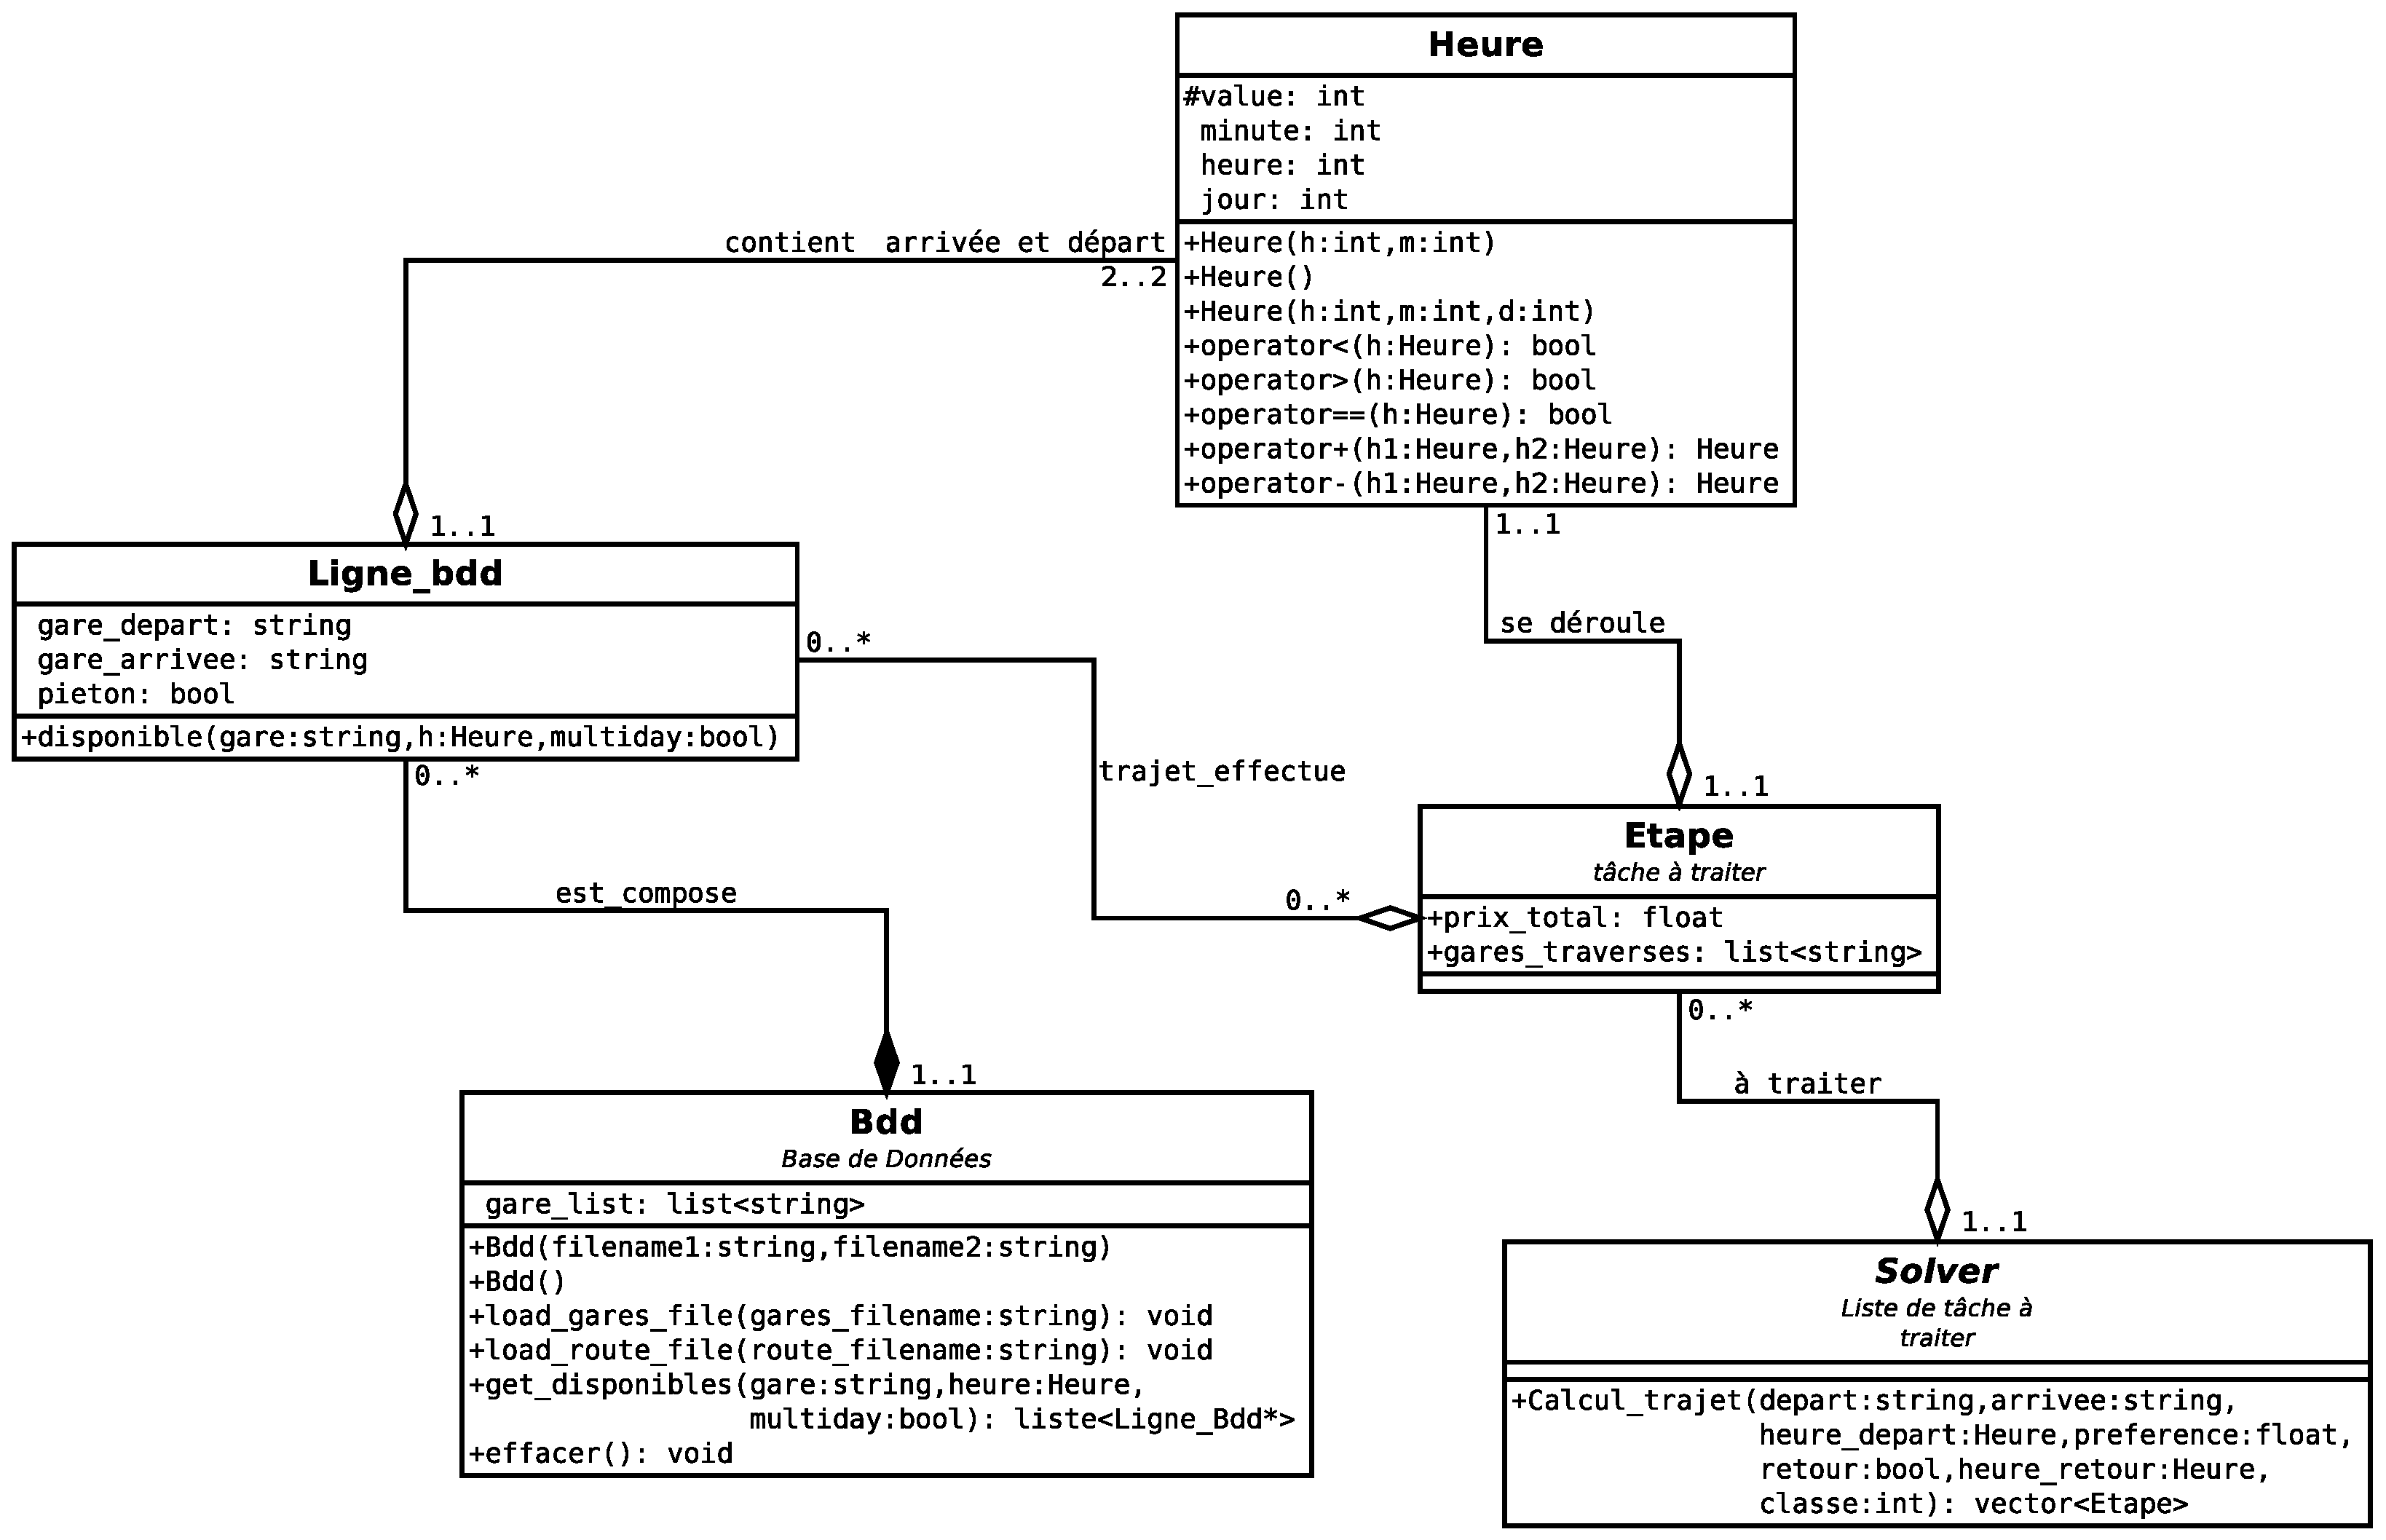
\includegraphics[width=\textwidth]{Diagram1.eps}
    \caption{Diagramme des classes (simplifié) de notre modèle}
    \label{diagclasse}
    \end{figure}
    

\chapter{Algorithme de Recherche}
\label{algorithme}
   
   
   
   \section{Algorithme principal}
    L'algorithme fonctionne de la façon suivante :\\
    \begin{itemize}
    \item une étape correspondant à la ville de départ et à l'heure de départ au plus tôt indiquée est créée puis ajoutée à la liste d'étape à traiter.
    \item jusqu'à ce qu'il n'y ait plus d'étape à traiter : \\
    \begin{itemize}
    \item on prend l'étape la plus intéressante de file de traitement.
    \item on regarde si la ville correspond à la destination, auquel cas on l'ajoute au "top X" si le trajet obtenu est plus intéressant qu'un des trajets déjà trouvé.
    \item si la ville ne correspond pas à la destination, on vérifie que la poursuite du chemin est pertinente en terme de temps/prix par rapport au "top X". Si ce n'est pas le cas, on supprime cette étape de la liste sans la traiter.
    \item sinon, si cette étape est intéressante, on regarde l'ensemble des trajets pouvant être effectués en partant de cette étape et pour chacune on crée une nouvelle étape à traiter (constituée du chemin déjà parcouru + le nouveau trajet).
    \end{itemize} 
    \end{itemize}
    
    \paragraph{}Dans notre implémentation actuelle, nous faisons le choix de traiter l'étape ayant la valeur (coût/temps) la plus faible.\\
    Ce choix nous amène à faire un parcours du graphe en pseudo-largeur en priorisant les étapes les plus intéressantes, à l'instar de l'algorithme de Dijkstra étudié en cours. L'établissement d'un premier chemin est plus long que dans le cas d'un parcours en profondeur (toujours traiter l'étape ajoutée), mais la qualité de ce chemin se veut très bonne, sinon la meilleure. Une fois le premier "TOPX" établi, nous pouvons arrêter de continuer certains chemins, avant même qu'ils n'aient atteints leurs destinations. Intérêt de trouver rapidement de bons chemins (heuristiques - méta-heuristiques) peut-être un facteur important sur le temps de résolution.
    
    
    
    
    
    \section{Cas d'aller-retour}
    D'après les contraintes du cahier des charges, un aller-retour doit être traité comme un trajet unique. Le cas d'un aller-retour se gère donc algorithmiquement de la même façon qu'un aller-simple, à la différence près qu'une fois la destination atteinte, nous vidons la liste des villes déjà parcourues, et nous réinjectons l'étape dans la file de traitement (en direction cette fois-ci de la ville de départ). Un chemin ne peut repartir de la ville d'arrivée avant l'heure de retour indiqué par l'utilisateur. En revanche, si un trajet arrive après l'heure souhaitée, il peut repartir immédiatement en direction de la ville d'origine. Un chemin est évalué sur l'ensemble de son trajet, depuis l'heure de départ effective (premier train) à l'heure de retour à la gare initiale. Il en est de même pour l'évaluation du coût de transport.
    
    
    
    
    \section{La mixité des critères}
    Le cahier des charges spécifie que le programme doit permettre à l'utilisateur de faire un choix quant aux critères qu'il souhaite minimiser en priorité : Le temps de trajet, le prix, ou un mixte des deux.\\
    Concernant les deux premières options, l'algorithme va simplement traiter en priorité le temps ou le prix et retenir dans le "top X" les solutions les plus intéressantes selon ce critère.\\
    Pour le critère de mixité, nous l'avons traité de façon différente dans l'interface graphique et dans l'interface console :\\
    \begin{itemize}
    \item pour l'\textbf{interface graphique} l'utilisateur peut choisir une valeur intermédiaire plus ou moins proche d'un critère ou d'un autre en faisant défiler une jauge. Plus la jauge sera vers le temps, plus le critère de temps sera considéré et inversement pour le prix. Le résultat de ce choix est une valeur entre 0 et 1, 0 correspondant à une priorité intégrale sur le prix et 1 sur le temps.\\
    \item pour l'\textbf{interface console}, l'utilisateur possède les même choix, le choix de la mixité n'est pas réglable, il retourne uniquement une valeur égale à $0.5$.
    \end{itemize}
    
    
\chapter{Résultats et Conclusions}
    \section{Résultats et interface}
        Vous trouverez des exemples de résultats et d'étapes d'exécution dans les figures \ref{screen1} \ref{screen2} (console) \ref{screen3} \ref{screen4} \ref{screen5} (graphique)
    
    
    
    \section{Les limites de l'algorithme}
    Le programme gère les cas d'aller-retour en tant que trajet unique. Dans le cas d'une minimisation du temps d'un trajet, le temps du trajet total évalué sera proche de l'écart entre le jour du départ et le jour du retour. Les résultats du "top X" auront donc des valeurs en temps importantes si on effectue le retour plusieurs jours après l'aller. Les contraintes de coupes ne seront donc plus efficaces dans ce cas-là, car la coupe s'effectue quand la valeur d'une étape dépasse la pire valeur du top X. Une grande partie des branches séparant le jour de départ et le jour de retour seront donc explorées. Cela explique que le programme peut prendre énormément de temps à la résolution sur de grandes instances. 
    
    
    
    \section{Améliorations possibles}
    \paragraph{}Pour résoudre le problème d'un aller-retour espacé prenant en compte le temps dans ses priorités, il faudrait évaluer l'aller et le retour de façon séparée ce qui permettrait de rendre les contraintes de coupes efficaces.
    \paragraph{}Une autre façon d'améliorer l'algorithme serait d'affiner la méthode de comparaison définissant la priorité des étapes à traiter. Pour cela on pourrait assigner à chaque ville une coordonnée GPS et traiter en priorité les trajets se rapprochant de la destination. Cela permettrait à la fois de se rapprocher très rapidement vers la destination et donc d'obtenir rapidement X résultats intéressants, ce qui rendra les contraintes de coupes beaucoup plus efficaces.  
 
 \begin{figure}[p]
    \centering
    \includegraphics[width=\textwidth]{screenshot4.png}
    \caption{Interface console}
    \label{screen1}
    \end{figure}
    
    \begin{figure}[p]
    \centering
    \includegraphics[width=\textwidth]{screenshot5.png}
    \caption{Interface console}
    \label{screen2}
    \end{figure}
    
    \begin{figure}[p]
    \centering
    \includegraphics[width=0.8\textwidth]{screenshot1.png}
    \caption{Interface graphique}
    \label{screen3}
    \end{figure}
     \begin{figure}[p]
    \centering
    \includegraphics[width=0.8\textwidth]{screenshot2.png}
    \caption{Interface graphique}
    \label{screen4}
    \end{figure}
     \begin{figure}[p]
    \centering
    \includegraphics[width=0.8\textwidth]{screenshot3.png}
    \caption{Interface graphique}
    \label{screen5}
    \end{figure}
\end{document}


